\subsection{Lexikální analýza}
\label{subsec:lexer}
Úlohou Lexikálního analyzátoru je rozpoznávat jazykové lexémy a reprezentovat
je jako tokeny.

Lexikální analyzátor je implementací deterministického konečného
automatu. Jediný nedeterministický případ nastává tehdy, když má automat načítat znak ve tvatu $\backslash$ddd.
Případ je vyřešen implementací interního čítače počtu číslic.

Lexikální analyzátor je rozdělen do tří modulů: \ic|lexer.c|, \ic|lexer_fsm.c| a \ic|token.c|
. Modul \ic|token.c| obsahuje implementaci abstraktního datového typu token. Modul \ic|lexer_fsm.c|
obsahuje implementaci deterministického konečného automatu. Modul \ic|lexer.c| poskytuje funkci
\ic|lexer_next_token|, která řídí činnost deterministického konečného automatu a
která vrací další token.

\vspace*{16px}
\begin{figure}[htbp]
    \centering
    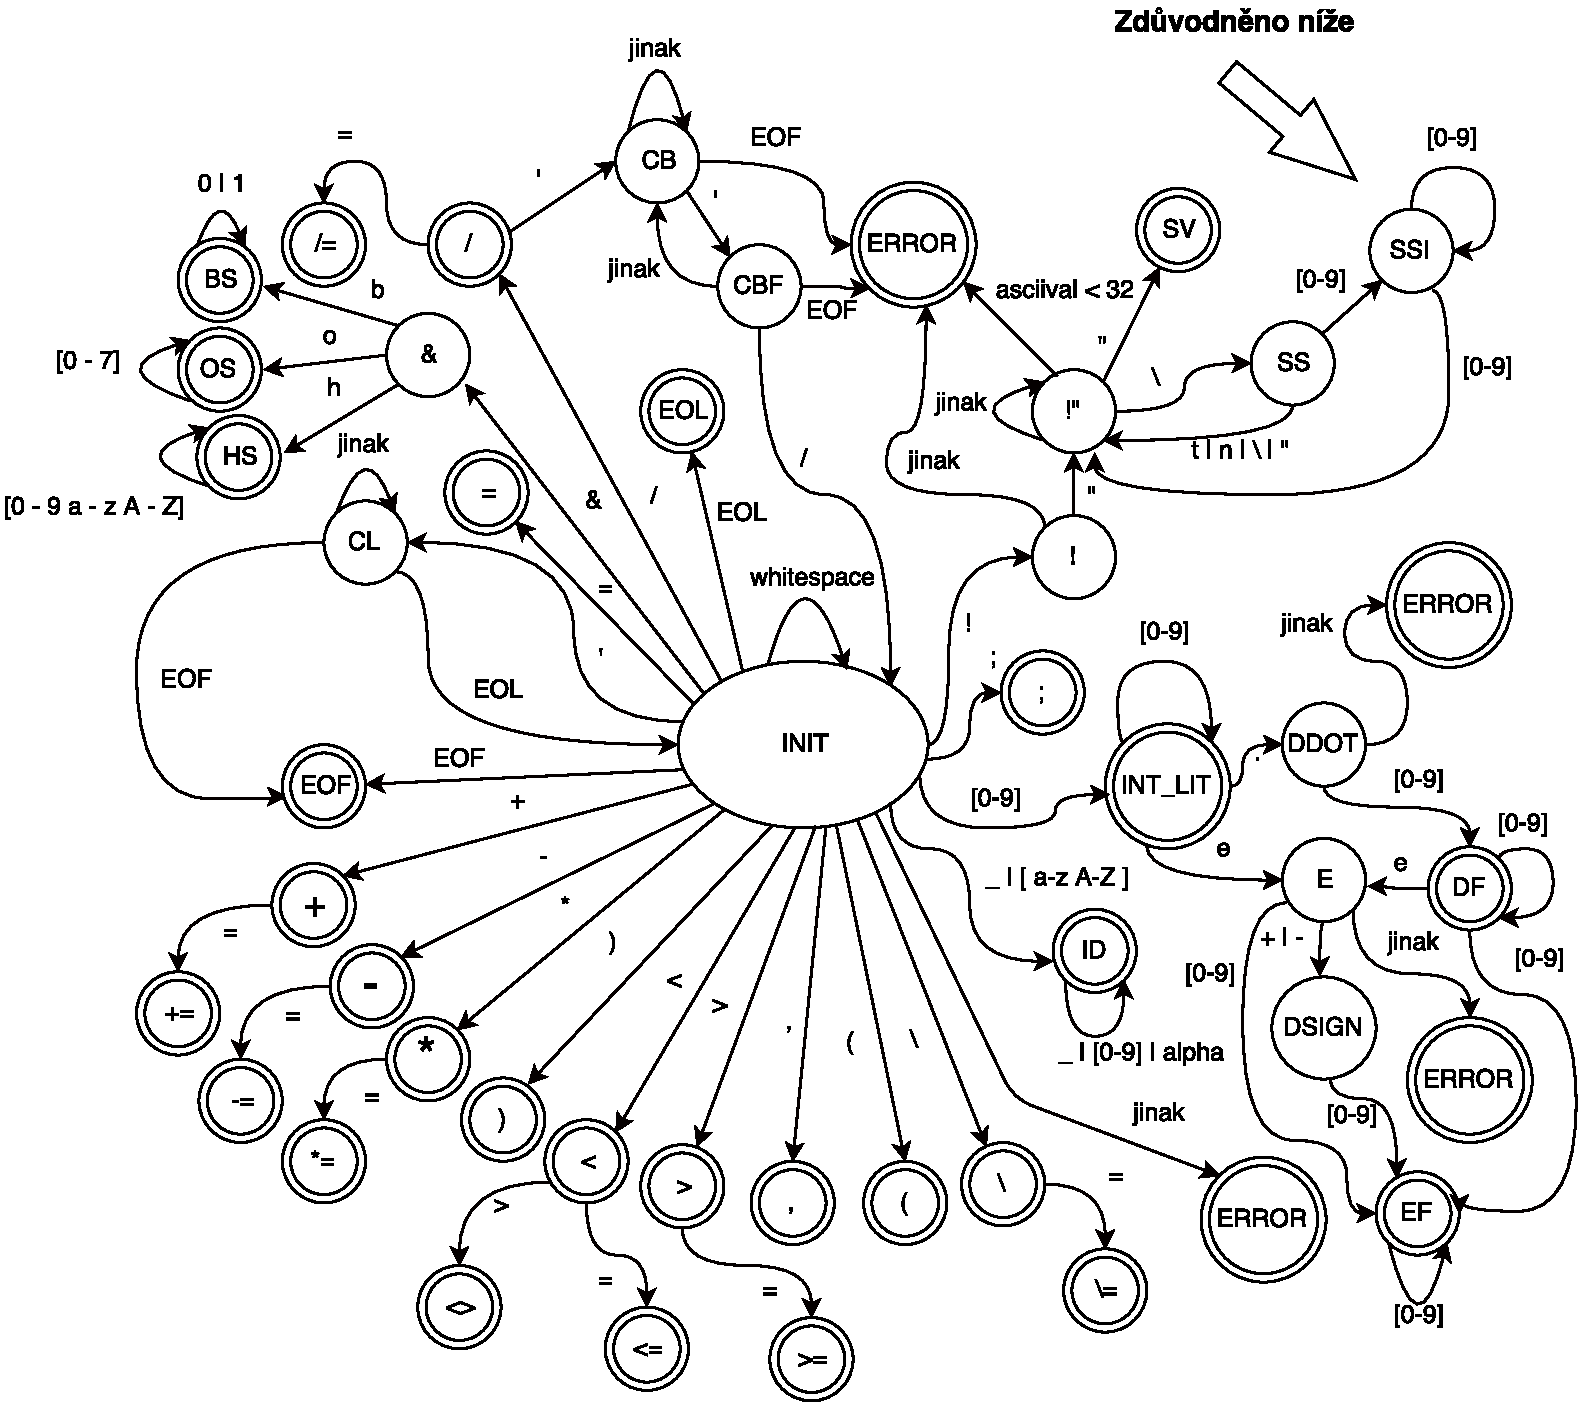
\includegraphics[width=1\textwidth, angle=0]{src/assets/automat.pdf}
\end{figure}

\subsection{Synataktická analýza}
Syntaxí řízený překlad je naimplementován v modulu \ic|parser.c|, pro syntaktickou analýzu programu jako takového je
použita SA shoda dolů, konkrétně metoda rekurzivního sestupu. Pro každé pravidlo z LL gramatiky existuje v tomto
modulu funkce realizující toto pravidlo.

Pro snažší zápis v jazyce C byl implementován poloautomatický systém generování funkcí reprezentující tato pravidla za pomocí maker.
Makra konkrétní pravidlo zavolají a zkontrolují jeho splnění. Pro kontrolu terminálu bylo naimplemntováno makro
\ic|CHECK_TOKEN(TOKEN_TYPE)|,
Pro zavolání pravidla bylo naimplementováno pravidlo \ic|CALL_RULE(NAME_OF_RULE);|.
Pro podmínečná volání pravidel poté makro ve stylu
\ic|CHECK_RULE(token_type == TOKEN_TYPE, NAME_OF_RULE, REWIND_AND_SUCCESS)| - Pri použití se zavolá pravidlo
\ic|NAME_OF_RULE| v případě, že je následující token typu \ic|TOKEN_TYPE| a jestliže bylo úspěšné, další načtený
token navrátí zpět a prohlásí volání za úspěšné.

Všechny pravidla pracují nad strukturou \ic|Parser|, která zapouzdřuje základní komponenty pro syntaxí řízený překlad.
Jedná se především od struktury \ic!ParserSemantic!, \ic!CodeConstructor! a \ic!Lexer!. První zmíněná zajištuje sémantické
kontroly programu; uchovává \emph{registr symbolů}, dočasné proměnné, pravidla pro implicitní konverze datových typů či
aktuální scénář SA. Konstruktor kódu je poté popsán v příslušné sekci \ref{subsec:code-constructor}, Lexer v sekci
\ref{subsec:lexer}.

Pro analýzu výrazů není analýza shora dolů příliš vhodná, proto byla
použita metoda zdola nahoru v našem případě založená na precedenční
syntaktické analýza implementovaná v souboru \ic|parser_expr.c|.

Přepínání mezi metodami je realizováno následujícím mechanismem. Na celý program je použita funkce \ic|parser_parse|
z modulu \ic|parser.c|. V případě že je jako neterminál očekáván výraz, je volána funkce \ic|parser_parse_expr|
z modulu \ic|parser_expr.c|, která provede precedenční syntaktickou analýzu výrazu.

\subsubsection{Gramatika}

\begin{enumerate}
\item <prog> $\rightarrow$ <body> <eols> EOF
\item <body> $\rightarrow$ <definitions> <scope> <shared\_variables\_declarations>
\item <body> $\rightarrow$ <definitions> <statement\_scope>

\item <definitions> $\rightarrow$ <eols> <definition> <definitions>
\item <definitions> $\rightarrow$ <eols> E

\item <definition> $\rightarrow$ <function\_declaration>
\item <definition> $\rightarrow$ <function\_definition>
\item <definition> $\rightarrow$ <shared\_variable\_declaration>

\item <function\_definition> $\rightarrow$ <function\_header> EOL <eols> <statements> END FUNCTION
\item <function\_declaration> $\rightarrow$ DECLARE <function\_header> EOL <eols>

\item <function\_header> $\rightarrow$ FUNCTION IDENTIFIER (<function\_params>) AS <type>

\item <function\_params> $\rightarrow$ E
\item <function\_params> $\rightarrow$ <function\_param> <function\_n\_param>

\item <function\_n\_param> $\rightarrow$ E
\item <function\_n\_param> $\rightarrow$ <function\_param> <function\_n\_param>

\item <function\_param> $\rightarrow$ IDENTIFIER AS <type>


\item <type> $\rightarrow$ INTEGER
\item <type> $\rightarrow$ BOOLEAN
\item <type> $\rightarrow$ STRING
\item <type> $\rightarrow$ DOUBLE

\item <statements> $\rightarrow$ E
\item <statements> $\rightarrow$ <statement\_single> EOL <eols> <statements>


\item <statement\_single> $\rightarrow$ <identifier\_assignment>
\item <statement\_single> $\rightarrow$ <input>
\item <statement\_single> $\rightarrow$ <return>
\item <statement\_single> $\rightarrow$ <print>
\item <statement\_single> $\rightarrow$ <condition>
\item <statement\_single> $\rightarrow$ <while\_>
\item <statement\_single> $\rightarrow$ <variable\_declaration>
\item <statement\_single> $\rightarrow$ <static\_variable\_declaration>
\item <statement\_single> $\rightarrow$ <scope>

\item <variable\_declaration> $\rightarrow$ DIM IDENTIFIER AS <type> <declaration\_assignment>
\item <declaration\_assignment> $\rightarrow$ E
\item <declaration\_assignment> $\rightarrow$ <assignment>

\item <shared\_variables\_declarations> $\rightarrow$ E
\item <shared\_variables\_declarations> $\rightarrow$ <shared\_variable\_declaration>
\item <shared\_variable\_declaration> $\rightarrow$ DIM SHARED IDENTIFIER AS <type> <declaration\_assignment>

\item <static\_variable\_declaration> $\rightarrow$ STATIC IDENTIFIER AS <type> <declaration\_assignment>

\item <return> $\rightarrow$ RETURN <expr>

\item <assignment> $\rightarrow$ <modify> <expression>
\item <modify> $\rightarrow$ +=
\item <modify> $\rightarrow$ -=
\item <modify> $\rightarrow$ *=
\item <modify> $\rightarrow$ /=
\item <modify> $\rightarrow$ $\backslash$=

\item <print> $\rightarrow$ PRINT <print\_expression> <print\_expressions>
\item <print\_expressions> $\rightarrow$ E
\item <print\_expressions> $\rightarrow$ <print\_expression> <print\_expressions>
\item <print\_expression> $\rightarrow$ <expression> SEMICOLON

\item <while\_> $\rightarrow$ DO WHILE <expression> EOL <eols> <cycle\_statements> LOOP

\item <input> $\rightarrow$ INPUT IDENTIFIER

\item <condition> -> IF <expr> THEN EOL <eols> <statements>
\item <condition\_elseif> <condition\_else> END IF
\item <condition\_elseif> -> E
\item <condition\_elseif> -> ELSEIF <expr> THEN EOL <statements> <condition\_elseif>

\item <condition\_else> -> E
\item <condition\_else> -> ELSE EOL <eols> <statements>

\item <eols> $\rightarrow$ E
\item <eols> $\rightarrow$ EOL <eols>

\end{enumerate}
\newpage
\subsection{Precedenční analýza výrazů}
Precedenční analýza je řízena precedenční tabulkou, kterou se vyhodnocuje pořadí zpracování tokenů. \ref{table:prec}
\ic|parser_expr_prec_table_data.c|. V tabulce se nachází jak binární, tak i unární mínus. 
Lexikální analyzátor nám ovšem poskytuje pouze jeden token mínus a proto se unární a binární mínus 
musí vyhodnotit podle kontextu. Precedenční analýza využívá se obousměrně vázaného seznamu, do kterého se ukládají terminály, 
precedenční symboly a neterminály. Pomocí redukčních pravidel, která jsou vypsána v příloze, se postupně výraz redukuje. 
Jelikož překladač je založen na přímém překladu, tak při redukování pomocí pravidel konstruktor kódu rovnou generuje kód programu.

\subsubsection{Redukční pravidla}

\begin{table}[htbp]
\centering
\label{Redukční pravidla}
\begin{tabular}{lll}
    $E \to i$ &  $E \to (E)$ & $E \to (E)$ \\
    $E \to (E)$ & $E \to i()$ & $E \to i(E)$\\
    $E \to i(E, E)$ & $E \to i(E, E, ...)$ &  $E \to E + E$\\
    $E \to E - E$ & $E \to E ~ / ~ E$ & $E \to E ~ \backslash ~ E$\\
    $E \to - E$ &  $E \to E = E$ & $E \to E <> E$\\
    $E \to E > E$ & $E \to E >= E$ & $E \to E < E$\\
    $E \to E <= E$ & $E \to NOT ~ E$ & $E \to E ~ AND ~ E$\\
    $E \to E ~ OR ~ E$ & & \\
\end{tabular}
\end{table}


\begin{table}[htbp]
\label{table:prec}
\centering
\caption{Precedenční tabulka}
\label{precedencni-tabulka}
\begin{tabular}{|l|l|l|l|l|l|l|l|l|l|l|l|l|l|l|l|l|l|l|l|l|}
\hline
& $un -$ & $*$ & $/$ & $\backslash$ & $+$ & $-$ & $=$ & $<>$ & $<$ & $<=$ & $>=$ & $>$ & $NOT$ & $AND$ & $OR$ & $($ & $)$ & $,$ & $i$ & \$ \\ \hline
$un -$ &$<$&$>$&$>$&$>$&$>$&$>$&$>$&$>$&$>$&$>$&$>$&$>$& x &$>$&$>$&$<$&$>$& x &$<$&$>$\\ \hline
$*$ &$<$&$>$&$>$&$>$&$>$&$>$&$>$&$>$&$>$&$>$&$>$&$>$&$<$&$>$&$>$&$<$&$>$&$>$&$<$&$>$\\ \hline
$/$ &$<$&$>$&$>$&$>$&$>$&$>$&$>$&$>$&$>$&$>$&$>$&$>$&$<$&$>$&$>$&$<$&$>$&$>$&$<$&$>$\\ \hline
$\backslash$ &$<$&$<$&$<$&$>$&$>$&$>$&$>$&$>$&$>$&$>$&$>$&$>$&$<$&$>$&$>$&$<$&$>$&$>$&$<$&$>$\\ \hline
$+$ &$<$&$<$&$<$&$<$&$>$&$>$&$>$&$>$&$>$&$>$&$>$&$>$&$<$&$>$&$>$&$<$&$>$&$>$&$<$&$>$\\ \hline
$-$ &$<$&$<$&$<$&$<$&$>$&$>$&$>$&$>$&$>$&$>$&$>$&$>$&$<$&$>$&$>$&$<$&$>$&$>$&$<$&$>$\\ \hline
$=$ &$<$&$<$&$<$&$<$&$<$&$<$&$>$&$>$&$>$&$>$&$>$&$>$&$<$&$>$&$>$&$<$&$>$&$>$&$<$&$>$\\ \hline
$<>$ &$<$&$<$&$<$&$<$&$<$&$<$&$>$&$>$&$>$&$>$&$>$&$>$&$<$&$>$&$>$&$<$&$>$&$>$&$<$&$>$\\ \hline
$<$ &$<$&$<$&$<$&$<$&$<$&$<$&$>$&$>$&$>$&$>$&$>$&$>$&$<$&$>$&$>$&$<$&$>$&$>$&$<$&$>$\\ \hline
$<=$ &$<$&$<$&$<$&$<$&$<$&$<$&$>$&$>$&$>$&$>$&$>$&$>$&$<$&$>$&$>$&$<$&$>$&$>$&$<$&$>$\\ \hline
$>=$ &$<$&$<$&$<$&$<$&$<$&$<$&$>$&$>$&$>$&$>$&$>$&$>$&$<$&$>$&$>$&$<$&$>$&$>$&$<$&$>$\\ \hline
$>$ &$<$&$<$&$<$&$<$&$<$&$<$&$>$&$>$&$>$&$>$&$>$&$>$&$<$&$>$&$>$&$<$&$>$&$>$&$<$&$>$\\ \hline
$NOT$ & x &$>$&$>$&$>$&$>$&$>$&$>$&$>$&$>$&$>$&$>$&$>$&$<$&$>$&$>$&$<$&$>$& x &$<$&$>$\\ \hline
$AND$ &$<$&$<$&$<$&$<$&$<$&$<$&$<$&$<$&$<$&$<$&$<$&$<$&$<$&$>$&$>$&$<$&$>$&$>$&$<$&$>$\\ \hline
$OR$ &$<$&$<$&$<$&$<$&$<$&$<$&$<$&$<$&$<$&$<$&$<$&$<$&$<$&$<$&$>$&$<$&$>$&$>$&$<$&$>$\\ \hline
$($ &$<$&$<$&$<$&$<$&$<$&$<$&$<$&$<$&$<$&$<$&$<$&$<$&$<$&$<$&$<$&$<$& = & = &$<$& x \\ \hline
$)$ &$>$&$>$&$>$&$>$&$>$&$>$&$>$&$>$&$>$&$>$&$>$&$>$&$>$&$>$&$>$& x &$>$&$>$& x &$>$\\ \hline
$,$ &$<$&$<$&$<$&$<$&$<$&$<$&$<$&$<$&$<$&$<$&$<$&$<$&$<$&$<$&$<$&$<$& = & = &$<$& x \\ \hline
$i$ & x &$>$&$>$&$>$&$>$&$>$&$>$&$>$&$>$&$>$&$>$&$>$& x &$>$&$>$& = &$>$&$>$& x &$>$\\ \hline
\$ &$<$&$<$&$<$&$<$&$<$&$<$&$<$&$<$&$<$&$<$&$<$&$<$&$<$&$<$&$<$&$<$& x & x &$<$& x\\ \hline
\end{tabular}
\end{table}


\subsection{Konstruktor kódu}
\label{subsec:code-constructor}
Konstruktor cílového kódu je komponenta překladače, která má za odpovědnost smysl a jednotlivé návaznosti vygenerovaného
tříadresného kódu.

Implementačně je založen na struktuře \ic|CodeConstructor|, obsahující pomocnou komponentu generátoru \ic|CodeGenerator|. Dále obsahuje následující položky:
\begin{description}[style=nextline]
    \item[zásobník návěští]
    \todo{je vůbec potřeba?}
    \item[zásobník návěští pro podmínky]
    Slouží pro uchování cílů skoků mezi jednotlivými větvemi podmínkového příkazu \ic|IF .. THEN|, \ic|ELSEIF ... THEN| a \ic|ELSE|.
    \item[zásobník návěští pro cykly]
    Obdobně jako záasobník pro podmínkové návěští, slouží tento zásobník pro uschování vygenerovaných návěští pro skoky na podmínku cyklu či mimo cyklus.
    \item[aktuální hloubku zanoření \texttt{SCOPE}]
    Určuje hlavní \ic|SCOPE| celého programu, podle které je poté generován cíl skoku do hlavního programu a vytvoření lokálního rámce.
    \item[zásobník počátečních instrukcí cyklu]
    Je určen pro uschování počátečních instrukcí cyklů \ic|LABEL|, které slouží jako zarážky pro vygenerování instrukcí před začátek bloku cyklu. Tedy například vygenerování instrukcí \ic|DEFVAR| před tělo cyklu - pro zamezení duplicitní definice.
    \item[hloubka zanoření řídících struktur]
    Definuje čítač pro automatické generování sekvence návěští pro cykly, podmínky, funkce a další použití.
    \item[seznam implicitních konverzí]
    Pomocný seznam typů instrukcí používaných pro konkrétní implicitní konverze operandů - je nutný pro plně automatickou kontrolu implicitních konverzí včetně generování konverzních instrukcí.
    \item[čítač vygenerovaných návěští]
    Interní čítač určený pro unikátní odlišení všech vygenerovaných instrukcí v rámci programu.
\end{description}

\subsection{Generátor cílového kódu}
Generátor kódu je nízkoúrovňová komponenta zastřešující skládání, validaci a vykreslování cílového kódu \ic|IFJcode17|.
Kontroluje generované instrukce a její operandy, tedy správné kombinace typů operandů (přístupy do rámců, konstatní
literály, návěští či datové typy) u konkrétních instrukcí.

Interní implementace spoléhá na \emph{obousměrně svázaný lineární seznam} struktur \ic|CodeInstruction|, které kromě
režijních ukazatelů uchovávají typ instrukce a ukazatele na až tři operandy, struktury \ic|CodeInstructionOperand|.
Tento seznam je uložen v datové struktuře \ic|CodeGenerator|, která dále obsahuje pole podpisů\footnote{Podpis
instrukce je složena z bitových masek definující povolené typy operandů a její textové reprezentace v kódu
\texttt{IFJcode17}.} instrukcí pro jejich validace.
Struktura \ic|CodeInstructionOperand| uchovává informace o svém typu a poté unii dat pro konkrétní typ operandu, tedy
ukazatel na proměnnou \ic|SymbolVariable|,
data konstanty \ic|CodeInstructionOperandConstantData| v unii s datovým typem nebo řetězec uchovávající název návěští.